\section{Seguimiento de carriles}

\begin{frame}\frametitle{Modelo cinemático}
  Considere la base móvil de la figura:
  \begin{figure}
    \centering
    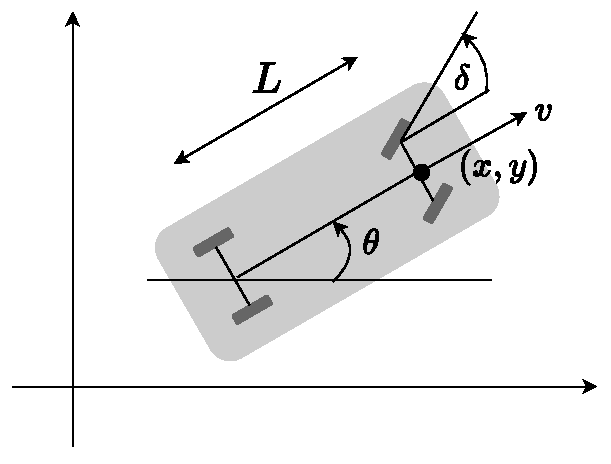
\includegraphics[width=0.3\textwidth]{Figuras/Ackermann.pdf}
  \end{figure}
  con
  \begin{itemize}
  \item $(x,y,\theta)$ la configuración en el plano de movimiento, considerando como centro el centro del eje delantero (tracción delantera)
  \item $L$ la distancia entre ejes de las llantas
  \item $v$ es la velocidad lineal del vehículo considerada como señal de entrada
  \item $\delta$ es el ángulo de las llantas delanteras (volante) también considerada como señal de control
  \end{itemize}
  El objetivo es determinar $v$ y $\delta$ de modo que le vehículo tenga determinado comportamiento.
\end{frame}

\begin{frame}\frametitle{Seguimiento de carriles}
  El seguimiento de carriles se puede hacer con base en las líneas detectadas. Considere la figura:
  \begin{figure}
    \centering
    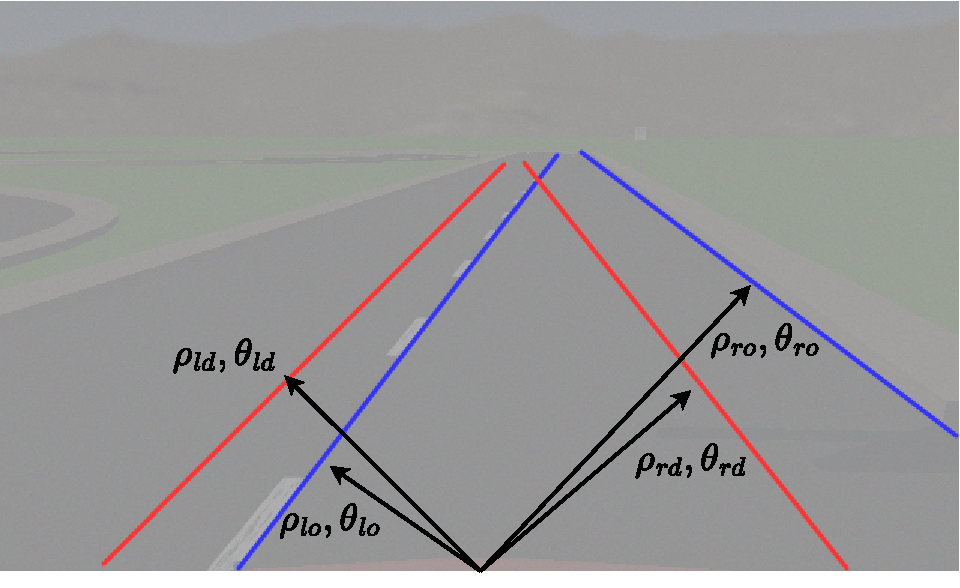
\includegraphics[width=0.5\textwidth]{Figuras/LineErrors.pdf}
  \end{figure}
  \begin{itemize}
  \item Las líneas azules son los bordes observados y las líneas rojas son las líneas que se deberían observar si el auto estuviera bien centrado y alineado en el carril.
  \item La diferencia entre los parámetros observados $(\rho_o,\theta_o)$ y los parámetros deseados $(\rho_d, \theta_d)$ se puede utilizar para calcular las señales $v,\delta$
  \end{itemize}
\end{frame}

\begin{frame}\frametitle{Seguimiento de carriles}
  \begin{itemize}
  \item El sterring $\delta$ se puede calcular con un control proporcional al error entre líneas deseadas y líneas observadas
  \item La velocidad lineal se puede calcular para que sea más pequeña cuando el auto esté girando
  \end{itemize}
  \begin{eqnarray*}
    \delta &=& K_\rho e_\rho + K_\theta e_\theta\\
    v &=& v_{max}(1 - k_\delta |\delta|)
  \end{eqnarray*}
  con
  \[
    e_\rho = \left\{ \begin{array}{lcl}
      \frac{1}{2}(\rho_{lo} - \rho_{ld} + \rho_{rd} - \rho_{ro}) & \textrm{si} & \rho_{lo}\neq 0\; , \; \rho_{ro} \neq 0\\
      (\rho_{lo} - \rho_{ld}) & \textrm{si} & \rho_{lo}\neq 0\\
      (\rho_{rd} - \rho_{ro}) & \textrm{en otro caso} & 
      \end{array}
    \right.\]
  \[
    e_\theta = \left\{ \begin{array}{lcl}
      \frac{1}{2}(\theta_{lo} - \theta_{ld} + \theta_{rd} - \theta_{ro}) & \textrm{si} & \theta_{lo}\neq 0\; , \; \theta_{ro} \neq 0\\
      (\theta_{lo} - \theta_{ld}) & \textrm{si} & \theta_{lo}\neq 0\\
      (\theta_{rd} - \theta_{ro}) & \textrm{en otro caso} & 
      \end{array}
    \right.\]
  y $K_\rho > 0$, $K_\theta > 0$, $k_\delta > 0$
\end{frame}

\begin{frame}[containsverbatim]\frametitle{Ejercicio 06 - Seguimiento de carriles}
  \begin{enumerate}
  \item Abra el archivo fuente del ejercicio 06 y agregue el siguiente código en la línea 27:
    \begin{lstlisting}[language=Python, firstnumber=27]
if rho_l != 0 and rho_r != 0:
    error_rho   = (rho_l   - goal_rho_l   + goal_rho_r   - rho_r)/2
    error_theta = (theta_l - goal_theta_l + goal_theta_r - theta_r)/2
elif rho_l != 0:
    error_rho   = rho_l   - goal_rho_l  
    error_theta = theta_l - goal_theta_l
else:
    error_rho   = goal_rho_r   - rho_r  
    error_theta = goal_theta_r - theta_r
steering = k_rho*error_rho + k_theta*error_theta
speed = max_speed*(1 - k_delta*abs(steering))
    \end{lstlisting}
  \item Abra una terminal y ejecute la simulación con el comando:
    \begin{lstlisting}[language=bash,numbers=none]
roslaunch eir2024 navigation_no_obstacles.launch
    \end{lstlisting}
  \item En otra terminal ejecute el ejercicio 05 (detección de carriles) con el comando:
    \begin{lstlisting}[language=bash,numbers=none]
rosrun eir2024 exercise05.py 
    \end{lstlisting}
  \end{enumerate}
\end{frame}

\begin{frame}[containsverbatim]\frametitle{Ejercicio 06 - Seguimiento de carriles}
  \begin{enumerate}
    \setcounter{enumi}{3}
  \item En otra terminal, ejecute el ejercicio 06 con el comando:
    \begin{lstlisting}[language=bash,numbers=none]
rosrun eir2024 exercise06.py _k_rho:=0.001 _k_theta:=0.01 _max_speed:=20
    \end{lstlisting}
  \item Observe el comportamiento del vehículo y sintonice las constantes $k_\rho$ y $k_\theta$.
  \item Cuando estén sintonizadas las constantes, pruebe con velocidades $v_{max}$ más altas.
  \end{enumerate}
\end{frame}

\begin{frame}\frametitle{Nubes de puntos}
  Las nubes de puntos son conjuntos de vectores que representan puntos en el espacio. Estos vectores generalmente tienen información de posición $(x,y,z)$. También pueden contener información de color $(x,y,z,r,g,b)$.
  \begin{figure}
      \centering
      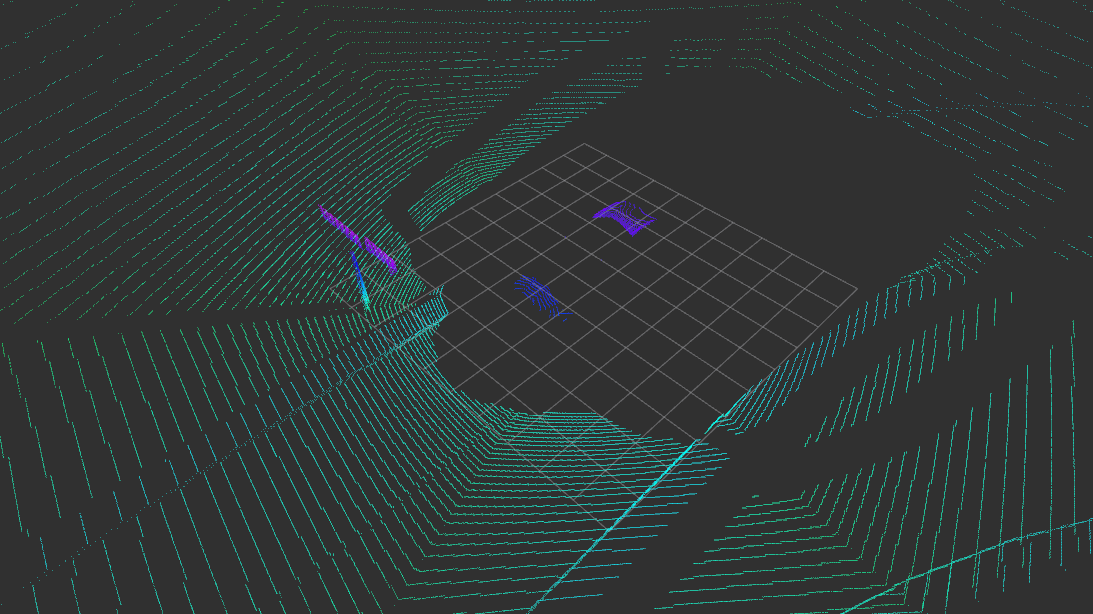
\includegraphics[width=0.5\textwidth]{Figuras/CloudExample.png}
  \end{figure}
  Son útiles para determinar la posición en el espacio de los objetos reconocidos.
  \begin{itemize}
  \item Para determinar si hay obstáculos frente al auto se puede emplear el sensor Lidar
  \item Este sensor genera una nube de puntos
  \item La nube se debe filtrar para suprimir el piso y los puntos del propio auto
  \end{itemize}
\end{frame}

\begin{frame}[containsverbatim]\frametitle{Ejercicio 07 - Detección de obstáculos}
  \begin{enumerate}
  \item Abra el código fuente del ejercicio 07 y agregue el siguiente código en la línea 44:
    \begin{lstlisting}[language=Python,firstnumber=44]
P = P[(P[:,2] > -1) & (P[:,2] < 0.3) ] #Filters points on floor and higher points
P = P[(P[:,0] > lower_x ) & (P[:,0] < upper_x ) & (P[:,1] < upper_y ) & (P[:,1] > lower_y )]      
    \end{lstlisting}
     \item Abra una terminal y ejecute la simulación con el comando:
    \begin{lstlisting}[language=bash,numbers=none]
roslaunch eir2024 navigation_static_obstacles.launch
    \end{lstlisting}
  \item En otra terminal ejecute el ejercicio 7 con el comando:
    \begin{lstlisting}[language=bash,numbers=none]
rosrun eir2024 exercise07.py
    \end{lstlisting}
  \item Mueva los vehículos en el simulador para verificar la correcta detección de obstáculos. 
  \end{enumerate}
\end{frame}

\begin{frame}\frametitle{Máquinas de estados}
  \begin{itemize}
  \item Sirven para representar procesos discretos determinísticos
  \item Están definidas por la tupla $(S, s_0, I, O, Z, F, F_o\)$:
    \begin{itemize}
    \item $S$ : Conjunto de estados
    \item $s_0 \in S$ : Estado inicial
    \item $I$ : Conjunto de entradas
    \item $O$ : Conjunto de salidas
    \item $Z \subset S$ : conjunto de estados finales (puede ser vacío)
    \item $F : S\times I \rightarrow S$ : Función de transición de estados (que generalmente se determina con una carta ASM)
    \item $F_o : \S \rightarrow O$ : Función de salida 
    \end{itemize}
  \item Se pueden usar para coordinar los comportamientos del vehículo 
  \end{itemize}
\end{frame}

\begin{frame}\frametitle{Ejercicio 08 - Rebase}
  
\end{frame}